% ===================================================================
% Presentación con Latex Beamer -> EN proceso de modificación -> CCF
% ===================================================================
\documentclass[9pt,xcolor=svgnames]{beamer}
%\documentclass[handout,xcolor=svgnames]{beamer} %Version imprimible
% -------------------------------------------------------------------
\usepackage{paquetes}
\usepackage{licencia}
% -------------------------------------------------------------------
\usepackage{modo}
% -------------------------------------------------------------------

% Comienza el documento
\begin{document}
% Tikz -> Imágenes
\tikzstyle{every picture}+=[remember picture]
% Entorno matemático
\everymath{\displaystyle}

% Transparencia de Inicio -> Título
\begin{frame}
  \titlepage
\end{frame}

\normalsize

% Transparencia de índice
\begin{frame}
 \frametitle{Índice} 
 %\transboxin
 \tableofcontents
\end{frame}

\section{Introducción}
\begin{frame}
    \frametitle{Introducción}

        \begin{block}{Juegos de conducción}
            \begin{itemize}
                \item Objetivo: llegar a la meta
                \item Zonas diferenciadas
                \item Adictivos
                \item Para todo tipo de jugadores
                %\item Cortos tiempos de juego
                \item Variados modos de juego
                \item No pasan de moda
            \end{itemize}
        \end{block}

    \begin{columns}
    
        \column{150px}
        %\begin{center}
                %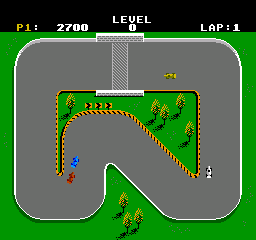
\includegraphics[scale=0.4]{imagenes/super_sprint.png}
        %\end{center}

        \begin{figure}
          \label{logo_latex}
          \begin{center}
            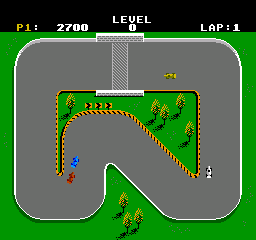
\includegraphics[scale=0.4]{imagenes/super_sprint.png}
          \end{center}
          Super Sprint - Atari (1986)
        \end{figure}
    
        \column{150px}
        \begin{figure}
          \label{logo_latex}
          \begin{center}
            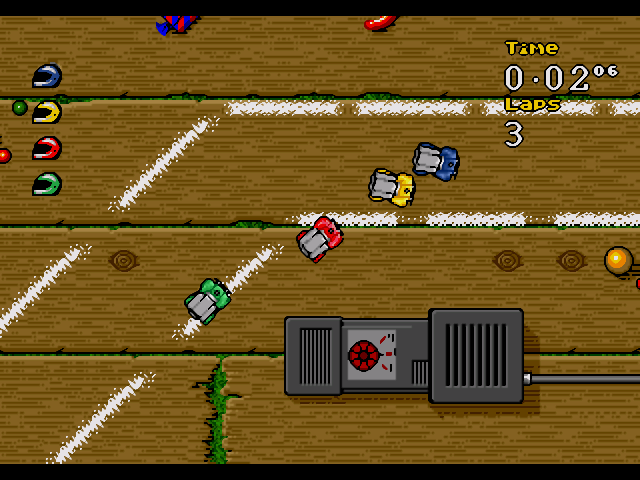
\includegraphics[scale=0.2]{imagenes/micromachines.png}
          \end{center}
          Micromachines - NES (1991)
        \end{figure}

    \end{columns}
    
\end{frame}

\begin{frame}
    \frametitle{Introducción}

    \begin{columns}
    
        \column{150px}
        \begin{block}{Zycars}
            \begin{itemize}
                \item Juego de conducción en 2D con vista cenital
                \item Tres modo de juego
                \item Uso de ítem durante las carreras
            \end{itemize}
        \end{block}

        \column{150px}
        \begin{figure}
          \label{logo_latex}
          \begin{center}
            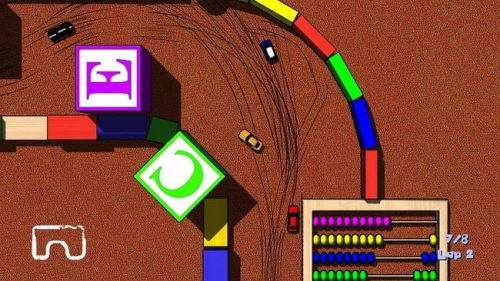
\includegraphics[scale=0.3]{imagenes/toy_cars.jpg}
          \end{center}
          Toy Cars - Xbox 360 (2011)
        \end{figure}
        
    \end{columns}


    \begin{block}{¿Por qué este proyecto?}
        \begin{itemize}
            \item Muy pocos juegos libre con las mismas características
            \item Interés por el mundo de los videojuegos
            \item Cursar la asignatura de Diseño de Videojuegos aumentó el interés por el desarrollo de estos
            \item Contribuir al mundo del software libre
        \end{itemize}
    \end{block}

\end{frame}

\begin{frame}
    \frametitle{Introducción}

    \begin{block}{Objetivos}
        \begin{itemize}
            \item Realizar un juego de coches completamente funcional
            \item Dificultad progresiva (adicción por aprendizaje)
            \item Competidores aceptables, que proponga un desafío superable
            \item Fácilmente ampliable
        \end{itemize}
    \end{block}

    \begin{columns}
    
        \column{200px}
        \begin{alertblock}{No es un simulador}
            \begin{itemize}
                %\item Movimiento básico de los coches
                %\item La colisiones se corrigen de forma sencilla
                \item Arcade, prima la diversión
                \item Coches fáciles de manejar
                \item Colisiones sólo paran a los coches (estrategia)
            \end{itemize}
        \end{alertblock}
        
        \column{100px}
        \begin{figure}
          \label{logo_latex}
          \begin{center}
            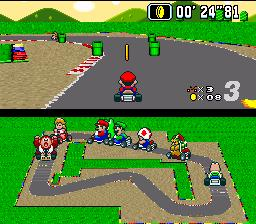
\includegraphics[scale=0.5]{imagenes/super_mario_kart.jpg}
          \end{center}
          Super Mario Kart - SNES (1992)
        \end{figure}
        
    \end{columns}
    
\end{frame}


\section{Descripción}

\section{Descripción}

\paragraph{}
El proyecto consiste en un juego de carreras en dos dimensiones con vista cenital, en el que se podrá competirá contra la 
inteligencia artificial. 
La idea es realizar un juego entretenido y dinámico, que estará compuesto por varios modos de juego.

\begin{figure}[H]
  \label{logo_zycars}
  \begin{center}
    
\includegraphics[scale=0.5]{imagenes/logo_zycars.png}
  \end{center}
  \caption{Descripción: Logo de Zycars}
\end{figure}

\section{Características del videojuego}

\paragraph{}
El videojuego ofrece una alternativa libre, gratuita y original para jugar a un juego de conducción en dos dimensiones. 
Las posibilidades que ofrece son las siguientes:

\subsection{Modos de juego}

\paragraph{}
En \emph{Zycars} tendremos distintos modos de juegos, en cada uno de ellos el
objetivo que habrá que llevar a cabo será distinto.
A continuación se describirán los distintos modos de juegos que tendrá el videjuego:

\subsubsection{Carrera rápida} 

\paragraph{}
El juego en el modo de carrera rápida ofrece la posibilidad de enfrentarnos a 3 personajes 
controlados por la inteligencia artificial, a lo largo de un circuito que
hayamos seleccionado previamente. El número de vueltas
que se realicen durante la carrera estarán a elección del jugador y se podrá elegir el número de las mismas a la hora de seleccionar
el circuito.

\subsubsection{Campeonato} 

\paragraph{}
En este modo de juego podremos competir contra 3 personaje controlados por la inteligencia artificial 
a lo largo de un campeonato completo, el cual habremos elegido previamente. 

\paragraph{}
El campeonato estará compuesto por cuatro circuitos y el número de vueltas a estos, también estarán a elección del jugador 
al igual que en el modo de juego explicado anteriormente.

\paragraph{}
Tras la conclusión de cada una de las carreras, los jugadores obtendrán una puntuación en función de la posición que haya 
obtenido. El jugador que mayor puntuación haya conseguido tras acabar los cuatro circuitos, se proclamará ganador del 
campeonato.

\subsubsection{Contrarreloj} 

\paragraph{}
En este último modo de juego y a diferencia de los dos anteriores, el jugador competirá solo sin ningún oponente.

\paragraph{}
El objetivo en este modo de juego será la realización de los circuitos ofrecidos y mejorar los tiempos de estos, ya sean la 
vuelta más rápida del circuito o el tiempo general. El número de vueltas que deberemos dar al circuito serán un total de tres, a
diferencia de los modos anteriores, no tendremos la posibilidad de modificar el valor.

\subsection{Elementos de juego}

\paragraph{}
En esta sección se hará una pequeña descripción de los distintos elementos que encontraremos a lo largo del juego, ya sean 
manipulados por los jugadores, o encontrados a lo largo de los circuitos.

\subsubsection{Personajes}
	
\paragraph{}
Los elementos básico del juego, habrá disponibles distintos personajes que tendrán asociado un 
vehículo característico a su personalidad y apariencia. Cada uno de ellos
tendrán distintas características, 
cosa a tener en cuenta a la hora de hacer nuestra elección por uno de ellos, como la velocidad, la aceleración y el giro.
	
\begin{figure}[H]
	\label{ejemplo_personaje2}
	\begin{center}
		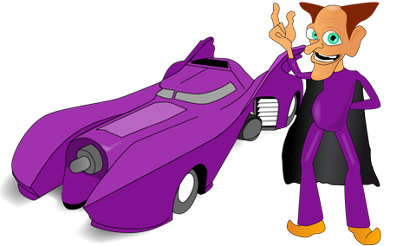
\includegraphics[scale=0.7]{imagenes/ejemplo_personaje2.png}
	\end{center}
	\caption{Descripción: Personaje de Zycars.}
\end{figure}

\subsubsection{Cajas de ítems} 

\paragraph{}
A lo largo de los circuitos en los que estemos compitiendo contra la inteligencia artificial, 
podremos encontrar distintas cajas que al colisionar con ellas nos proporcionen
aleatoriamente una habilidad o ítem que nos
ayuden en la competición contra nuestros rivales.

\begin{figure}[H]
	\label{item_box}
	\begin{center}
		
\includegraphics[scale=1]{imagenes/items/item_box.png}
	\end{center}
	\caption{Descripción: Caja de ítem.}
\end{figure}

\subsubsection{Tipos de ítems}

Los ítems que podremos obtener a partir de la caja de ítems, los podremos diferenciar principalmente en tres tipos:

\begin{description}
	\item \textbf{Ataques a distancia} Estos nos permitirán lanzar ataques
        de forma que podamos interceptar a los competidores que 
	se encuentres lejos de nosotros.
	
	\item \textbf{Obstáculos} Estos nos permitan dejar obstáculos en el
        recorrido, que reduzcan nuestra velocidad considerablemente
	o aquellos que al pasar por encima perdamos completamente el control de nuestro vehículo por unos instantes de tiempo.
	
	\item \textbf{Velocidad} Estos nos darán la opción de aumentar nuestra velocidad durante un pequeño intervalo de tiempo.
\end{description}

\section{Colaboradores}

\paragraph{}
Todo el apartado del proyecto referente a la programación del mismo se ha realizado de forma individual. En cambio, otros apartados
como el diseño gráfico, se ha contado con la colaboración de otra persona, y la música se ha obtenido de internet, concretamente 
de Jamendo, la página de música libre publicadas bajo licencias Creative Commons. Los créditos de juego son los siguientes:

\begin{description}
    \item [Desarrollador] José J. Marente Florín
    \item [Diseñador Gráfico] David Nieto Rojas
    \item [Música] Bob Wizman, Pirato Ketchup, Los Cadaver, The Wavers, Zamalska 
\end{description}


\section{Calendario}
\begin{frame}
    \frametitle{Planificación}

        \begin{block}{Propuesta del PFC}
            A finales de Mayo del 2010 se comenzó a plantear que se podía realizar como proyecto fin de carrera. 
            Tuvo lugar las reuniones con el tutor, con el fin de obtener distintas ideas. Finalmente entre todas las ideas
            propuestas se decidió realizar este proyecto.
        \end{block}
        
        \begin{block}{Tiempo de desarrollo}
            En septiembre de 2010 se comenzó el desarrollo, acabando aproximadamente a finales de Junio de 2011.
        \end{block}

\end{frame}

\begin{frame}
    \frametitle{Planificación}
        
        \begin{block}{Fases}
        Durante el periodo de desarrollo tuvieron lugar las distintas fases:
            \begin{itemize}
                \item \textbf{Fase de análisis}: indentificación de las necesidades del software.
                \item \textbf{Fase de diseño}: diseño de todo el sistema.
                \item \textbf{Fase de aprendizaje}: familiarización con el lenguaje python y la biblioteca pygame.
                \item \textbf{Fase de desarrollo}: implementación de todo los obtenido en la fase de diseño. Fase más larga.
                \item \textbf{Pruebas y correcciones}: pruebas necesarias para comprobar el correcto funcionamiento. En paralelo a
                la fase de desarrollo
                \item \textbf{Redacción de la memoria}: realización de la memoria final. 
            \end{itemize}
        \end{block}

\end{frame}

\begin{frame}
    \frametitle{Diagrama de Gantt I}

        \begin{center}
                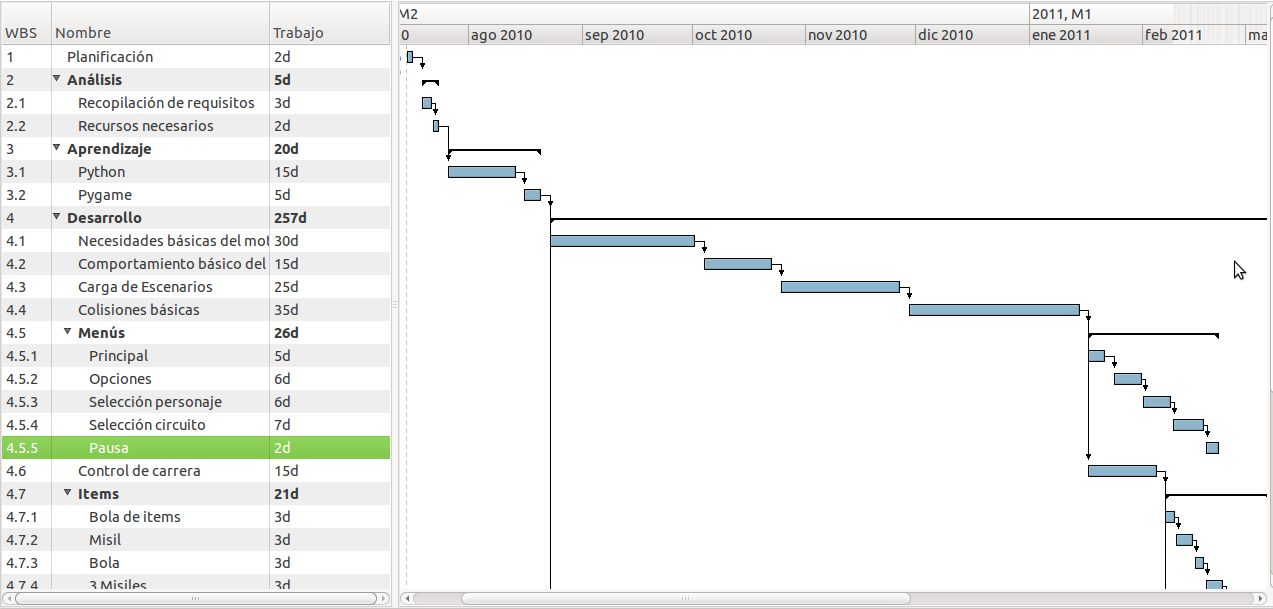
\includegraphics[scale=0.25]{imagenes/gant1.png}
        \end{center}
\end{frame}

\begin{frame}
    \frametitle{Diagrama de Gantt II}
        \begin{center}
                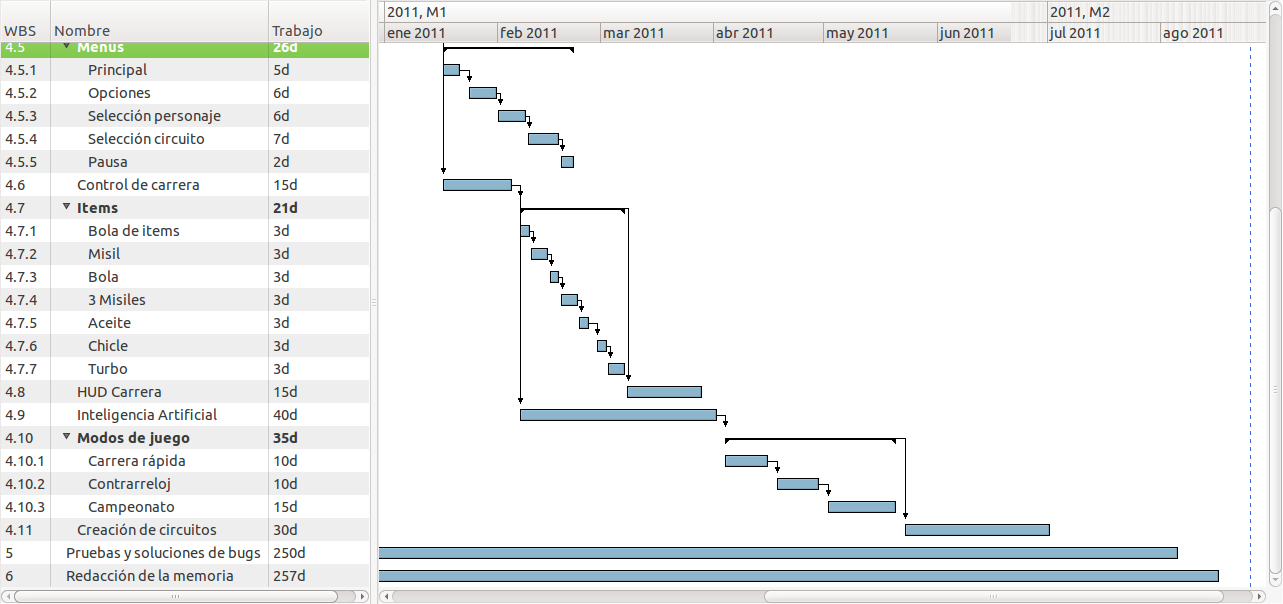
\includegraphics[scale=0.25]{imagenes/gant2.png}
        \end{center}
\end{frame}


\section{Implementación}
\begin{frame}
    \frametitle{Separar datos del código}

        En todo momento se ha procurado separar todos los datos de los personajes, circuitos y menús, del código
        fuente.\\
        \begin{block}{Ventajas}
            \begin{itemize}
                \item No es necesario saber programar para realizar cambios sobre cualquier parámetro.
                \item Cualquier persona puede ampliar el juego con nuevos personajes y nuevos circuitos, siguiendo
                los manuales creados para ello.
            \end{itemize}
        \end{block}
        \begin{block}{Solución}
            \begin{itemize}
                \item Todo se lee de ficheros XML
            \end{itemize}
        \end{block}

\end{frame}

\begin{frame}
    \frametitle{Formato de circuitos}

    \begin{block}{Mapas de tiles}
        Tile: imagen cuadrada, rectangular o hexagonal, utilizada para generar imágenes de mayor complejidad.
    \end{block}   
    
    \begin{block}{Editor de mapas: Tiled}
    Proporcionaba todas las necesidades básicas, 
    como una sencilla edición y creación de niveles, así como la gestión de capas,
    para poder poner elementos en el circuito a un nivel superior o inferior.\\
    Para ello se debía crear una imagen con todos los tiles que compondrían un circuito (tileset).\\
    Genera como resultado un XML.
    \end{block}   

    \begin{block}{Inconveniente}
        No permitia indicar de forma sencilla que tiles eran atravesables, colisionables o de cualquier otro tipo.
    \end{block}

\end{frame}

\begin{frame}
    \frametitle{Formato de circuitos}

        \begin{block}{Solución}
        Una imagen extra con las mismas características, donde los tiles sera de un único color, en función del tipo
        que estos sean.
        \end{block}

        \begin{center}
                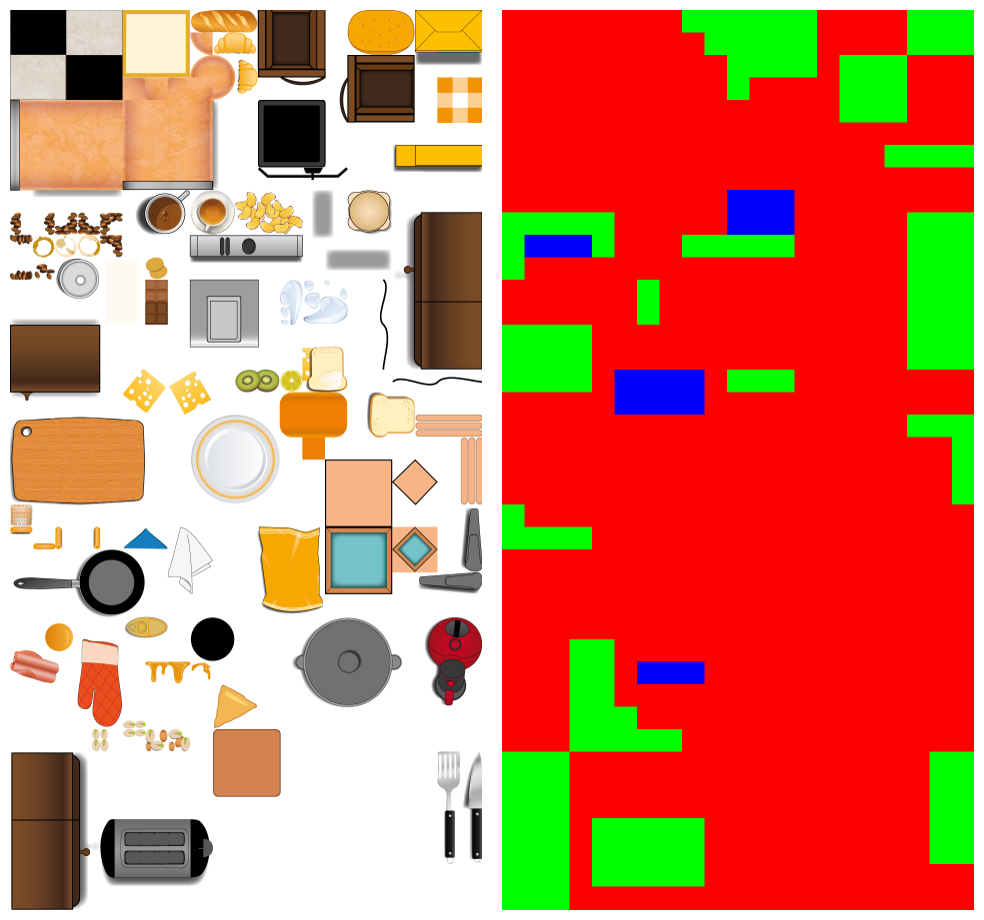
\includegraphics[scale=0.15]{imagenes/tileset-collisionmap.png}
        \end{center}
        

\end{frame}

\begin{frame}
    \frametitle{Colisiones}
    
    Una de las cosas más básicas en cualquier tipo de juego.

    \begin{block}{Colisión con el escenario}
        \begin{itemize}
            \item Detectamos si atravesamos algún tile no atravesable
            \item Si es así corregimos la posición del coche en según la dirección, sentido y lado del tile por
            el que colisione
            \item En el caso de que el tile sea de tipo realentizador, diminuimos la velocidad del coche
        \end{itemize}
    \end{block}

    \begin{center}
        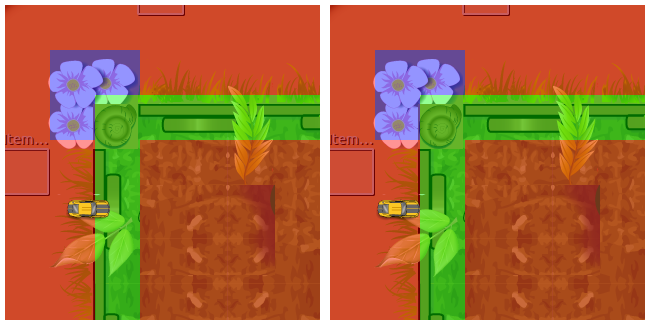
\includegraphics[scale=0.3]{imagenes/colision1-colision2.png}
    \end{center}
\end{frame}

\begin{frame}
    \frametitle{Colisiones}
    
    \begin{block}{Colisión entre vehículos}
        \begin{itemize}
            \item De forma similar a la colisión con el escenario
            \item Cuando se detecta la colisión se corrige la posición de los vehículos, en función la dirección, 
            sentido y lado del tile por el que colisionen
        \end{itemize}
    \end{block}
    
    \begin{block}{Colisión entre vehículos e ítems}
        \begin{itemize}
            \item Si es un ítem de ataque a distancia, destruiremos dicho ítem y cambiaremos el estado del coche con el que
            colisione
            \item Si el ítem es un obstaculo, cambiaremos el estado del coche en función del tipo de ítem
        \end{itemize}
    \end{block}

\end{frame}

\begin{frame}
    \frametitle{Inteligencia artificial}
    Otro de los aspectos más importante de un videojuego de las características de Zycars, es la
    inteligencia artificial, ya que en dos de los tres modos de juegos disponibles el objetivo es obtener la
    mejor clasificación posible, por delante de los demás coches controlados por el ordenador

        \begin{block}{Habilidades}
            \begin{itemize}
                \item Realización del recorrido: debe ser capaz de realizar los 
                recorridos de los circuitos.
                \item Lanzamiento de ítems: también debe poder usar los ítems que reciba de las bolas de ítems.
            \end{itemize}
        \end{block}
\end{frame}

\begin{frame}
    \frametitle{Realización del recorrido. Algoritmo A*}

    Aprovechando que tenemos un circuito creado por tiles y que podemos saber en todo momento en el tile 
    actual que se puede encontrar cualquiera de los competidores, se decidió implementar el 
    algoritmo de búsqueda A*.

        \begin{block}{Objetivo}
        Buscar el camino más corto y óptimo, en el caso de que exista, desde
        un nodo origen, hasta un nodo destino. A la hora de buscar dicho camino se tienen en cuenta factores
        como, el valor heurístico que poseen cada uno de los nodos, así como el coste real del recorrido.
        \end{block}

        \begin{block}{Parámetros}
        Los parametros que se tienen en cuenta en cada uno de los nodos.
            \begin{itemize}
                \item h’(n) es el valor heurístico del nodo actual n, hasta el final
                \item g(n) el coste real del camino desde el origen al nodo actual
                \item Función de evaluación: f(n) = g(n) + h’(n)
            \end{itemize}
        \end{block}

\end{frame}

\begin{frame}
    \frametitle{Realización del recorrido. Algoritmo A*}

        \begin{block}{Estructuras diferenciadas}
            \begin{itemize}
                \item Lista de abiertos: nodos por los que aún no se han pasado
                \item Lista de cerrados: nodos por los que ya se han pasado
            \end{itemize}
        \end{block}

        \begin{block}{Funcionamiento}
            Partiendo de un nodo en el que nos encontramos actualmente:
            \begin{enumerate}
                \item Obtenemos vecinos
                \item Comprobamos que no esten en abiertos ni cerrados
                \item Si alguno esta en abiertos, comprobamos su f(n), si es menor lo sustituiremos
                \item Introducimos en abiertos los que cumplan las condiciones
                \item Obtener de abiertos el nodo que tenga un f(n) menor y comenzamos de nuevo todo el proceso.
                \item Una vez lleguemos al nodo objetivo, detenemos la búsqueda y devolvemos el camino completo.
            \end{enumerate}
        \end{block}

\end{frame}

\begin{frame}
    \frametitle{Realización del recorrido. Algoritmo A*}

        Aplicación en Zycars

        \begin{center}
                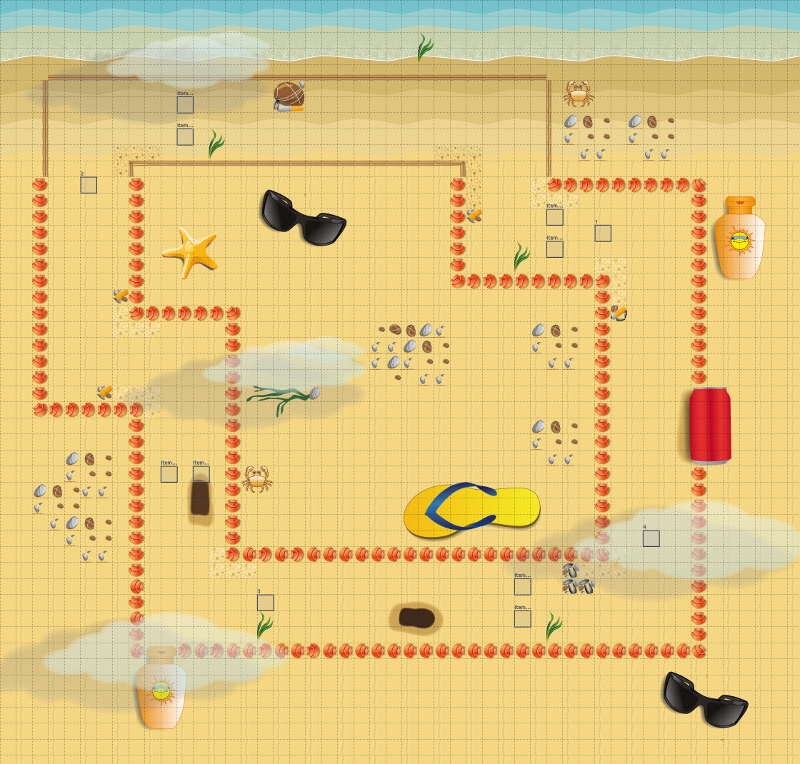
\includegraphics[scale=0.3]{imagenes/ia_check.png}
        \end{center}
        
\end{frame}

\begin{frame}
    \frametitle{Lanzamientos de ítems}

    Capaz de lanzar los ítems disponibles a los largo del juego, según las
    distintas situaciones en la que se encuentre.

        \begin{block}{Solución}
        Se eligió una forma muy sencilla y eficiente a la hora de realizarlo. Para ello cada
        vehículo controlado por la inteligencia artificial, tiene tanto un segmento que va desde el centro del
        coche hacia unos píxeles por delante de la posición actual del vehículo, como otro segmento que
        también va desde el centro pero uno píxeles atrás de la posición del vehículo.
        \end{block}

        \begin{center}
                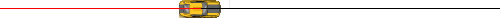
\includegraphics[scale=0.5]{imagenes/ia_segmentos.png}
        \end{center}

\end{frame}


\section{Herramientas}
\begin{frame}
    \frametitle{Herramientas}

        \begin{block}{Lenguaje de programación: Python}
        Oportunidad perfecta para aprender un nuevo lenguaje de programación.\\
        Entre sus principales características:
            \begin{itemize}
                \item Sintaxis limpia y que favorece un código legible.
                \item Multiplataforma
            \end{itemize}
        Destacar que se han obtenido unos resultado muy satisfactorios y ha cumplido todas las expectativas esperadas.

        \end{block}

        \begin{block}{Biblioteca gráfica: Pygame}
        Wrapper de la biblioteca SDL, de C/C++, para Python, por lo que tiene todas las virtudes de dicha biblioteca:
            \begin{itemize}
                \item Multiplataforma compatible con Microsoft Windows, GNU/Linux, Mac OS y QNX
                \item Muy completa (imágenes 2D, sonido, música y entrada estándar)
                %\item Usada durante la asignatura de Diseño de Videojuegos, características conocidas.
            \end{itemize}
        \end{block}

\end{frame}

\begin{frame}
    \frametitle{Herramientas}

        \begin{block}{Analizador de código: Pylint}
        Analiza el código Python en busca de errores y señales de mala calidad.\\
        La nota obtenida en el código del proyecto es de 8.25 sobre 10.
        \end{block}

        %\begin{block}{Sistema de control de versiones: Subversion}
        \begin{block}{Forja del proyecto}
        Alojado en el sistema que proporciona Google Code, bajo el sistema de control de versiones subversion.
            \begin{itemize}
                \item Pública
                \item Descargas para windows, linux y código fuente
                \item Página inicial (vídeos de demos, descripción, capturas, etc)
            \end{itemize}
        \end{block}

        \begin{block}{Documentación del código: Doxygen}
            \begin{itemize}
                \item Permite la documentación sencilla y legible de todo el código
                \item Generando en varios formatos como puede ser HTML o PDF
            \end{itemize}
        Para python existe la herramienta Doxypy.
        %que nos permite usar la convención de comentarios de Python y adaptarlos a Doxygen.
        \end{block}

\end{frame}



\section{Conclusiones}

\paragraph{}
En esta sección se comentarán las distintas conclusiones que se han obtenido tras la finalización del proyecto \emph{Zycars}.

\paragraph{}
En primer lugar comentar que es el primer proyecto de estas características al que me enfrento en solitario. Es evidente que su
realización no me ha dejado indiferente. No ha sido fácil construir una idea clara sobre lo que se quería hacer. Así como
solucionar los distintos problemas que han ido apareciendo a lo largo del desarrollo de este.

\paragraph{}
También decir que el proyecto me ha ocupado bastante más tiempo del esperado en un principio. Tuve muchos problemas y alguna que 
otra duda en algunas fases del desarrollo de proyecto, que me tuvieron bloqueado durante un tiempo hasta encontrar la solución
más adecuada para estos. A pesar de todo, estoy muy satisfecho con el resultado que se ha obtenido.

\paragraph{}
Se puede decir que el proyecto goza de buena calidad. Se ha intentado hacer un
software sencillo, intuitivo, fácil de manejar y 
entretenido para el jugador. Algo esencial para un juego de estas características, en el que se busca que cualquier persona
pueda echar algún rato de su tiempo libre y qué menos que disfrute durante ese tiempo.

\paragraph{}
Durante el desarrollo del proyecto se han aprendido muchísimas cosas: como hacer distintas ramas de desarrollo, plantear y crear
calendarios, usar las herramientas adecuadas, hacer decisiones importantes para el desarrollo de este, documentación del 
código, organización, etc. Ya que durante la carrera se han realizado distintas prácticas y trabajos de complejidad, pero nada
con el tamaño y duración que requiere un Proyecto de fin de carrera. Una vez finalizado este creo que tengo la experiencia necesaria
para afrontar otro proyecto con buenos resultados.

\paragraph{}
Entre las distintas herramientas, \LaTeX es una de esas en las que he aumentado mis conocimientos durante la realización de la 
memoria y gracias al compañero Pablo Recio por la plantilla facilitada para la realización de la memoria del proyecto, que sin duda
ha evitado muchos problemas.

\paragraph{}
Puedo decir que he aprendido un nuevo lenguaje de programación, como es \emph{Python}, ya que, que mejor forma de aprender un 
nuevo lenguaje, que realizar un proyecto con este.

\paragraph{}
He aprendido a usar con bastante soltura la biblioteca \emph{Pygame}, gracias tanto a la documentación de la página oficial, como
a la traducción disponible en Loserjuegos.

\paragraph{}
En definitiva, este proyecto me ha hecho madurar como persona y estudiante. He aprendido a buscar bibliografía, opiniones en otras
personas, compartir ideas, seguir un horario, cumplir una fechas de entrega y enfrentarme a un proyecto de estas características.

\section{Mejoras y ampliaciones}

\paragraph{}
Las posibles mejoras y ampliaciones que se podrían añadir al proyecto en futuras versiones, se comentan a continuación:

\begin{itemize}
    \item \textbf{Modo de dos jugadores}: añadir un nuevo modo de juego que nos permitiera jugar contra otra persona en el mismo
    ordenador. De forma que la pantalla quedaría dividida en dos.
    
    \item \textbf{Modo en red}: también sería una buena idea añadir un modo de
    juego en el que pudiésemos jugar en red contra otros
    oponentes. Este modo sería más conveniente que el modo de dos jugadores, ya que dos personas jugando en un mismo ordenador
    puede llegar a ser incomodo.
    
    \item \textbf{Mayor diversidad de ítems}: implementar nuevo ítems de distintos tipos dentro de los tipos prefijados, como 
    podrían ser misiles inteligentes o ítem que afectaran a todos los demás oponentes a la vez, como que estos encogieran por
    ejemplo. Este es un campo que en el obtendríamos muchas ideas.
    
    \item \textbf{Soporte para varias resoluciones}: añadir soporte para varias resoluciones sería algo muy como para aquellas 
    personas con pantalla muy pequeñas, como pueden ser los usuarios de netbooks, o también para persona con grande resoluciones
    que desean una ventana de juego mayor.
    
    
    \item \textbf{Más y mejores sonidos}: debido a que no se ha tenido la ayuda de ningún técnico de sonido, este es un aspecto en el que el
    juego escasea bastante, ya que encontrar sonidos que concordaran con la temática del juego, era un poco complicado.
\end{itemize}


%\section{Mejoras y ampliaciones}
%\begin{frame}
    \frametitle{Mejoras y Ampliaciones}

        \begin{block}{Posibles mejoras y ampliaciones:}
            \begin{itemize}
                \item \textbf{Modo dos jugadores}:  nuevo modo de juego que nos permitiera jugar contra otra
                persona en el mismo ordenador. Pantalla quedaría dividida en dos.

                \item \textbf{Modo en red}: modo de juego para jugar en red contra otros oponentes. 
                Más conveniente que el modo de dos jugadores, ya 
                que dos personas jugando en un mismo ordenador puede llegar a ser incomodo.
                
                \item \textbf{Soporte para varias resoluciones}: cómodo
                para personas con pantalla muy pequeñas, como usuarios de netbooks, o
                también para persona con grandes resoluciones que desean una ventana de juego mayor.
                
                \item \textbf{Grabación de las mejores vueltas}: opción que permitiera grabar la vuelta
                más rápida de cada uno de los circuitos, almacenándolas en un fichero, y poder visualizarlas
                posteriormente.
                
            \end{itemize}
        \end{block}
        
\end{frame}


\section{Bibliografía}
\begin{frame}
    \frametitle{Bibliografía recomendada}
    \begin{thebibliography}{5}
        \beamertemplatearticlebibitems
            \bibitem{Python}	
            Página de \emph{Python}
            \newblock http://www.python.org/
            
            \bibitem{PyGTK}
            Página oficial sobre \emph{Pygame}
            \newblock http://www.pygame.org/
             
        \beamertemplatebookbibitems
            \bibitem{UML}
            Larman, Craig
            \newblock Applying UML and Patterns, 3ª Edición. Prentice Hall, 2004.
            
            \bibitem{Dive into Python}
            Pilgrim, Mark
            \newblock Dive into Python. Appress, 2004.
    \end{thebibliography}
\end{frame}

\begin{frame}
    \frametitle{Demostración}
    
    \begin{center}
        {\Huge Demostración de Zycars}
    \end{center}
    
    \begin{center}
        
\includegraphics[scale=0.25]{imagenes/logo_zycars.png}
    \end{center}

\end{frame}

\begin{frame}
    \frametitle{Esto es todo}
    
    \begin{center}
        {\Huge Gracias por su atención}\\
        \bigskip
        {\huge ¿Preguntas?}\\
        \bigskip
        {\LARGE http://code.google.com/p/zycars/}
    \end{center}

\end{frame}


%\section{Preguntas}

\end{document}
  
